\chapter{Implementación de la etapa de control}
\label{implementacion-control}

\section{Introducción}

En este capítulo se sintetiza e implementa la estrategia de control diseñada en el capítulo anterior. Debido a las características del lenguaje de programación a utilizar, los componentes del lazo de control deben ser programados individualmente, para después ser ensamblados en el sistema de control diseñado. Debido a esta propiedad de VHDL, además de la programación de cada componente, se realiza una simulación o \emph{test bench} para corroborar su correcto funcionamiento. Las herramientas utilizadas aquí fueron el entorno de desarrollo Xilinx ISE\textsuperscript\textregistered \hspace{0.6pt} y los simuladores de código HDL ISim\textsuperscript\textregistered \hspace{0.6pt} y ModelSim\textsuperscript\textregistered\hspace{0.6pt}, los cuales fueron descritos en el Capítulo \ref{cap-fpga}, Sección \ref{desarrollo-fpga}.

\section{Placa de desarrollo a utilizar}

\begin{wrapfigure}{r}{0.42\textwidth}
    \vspace{-15pt}
    \begin{center}
      \includegraphics[width=0.39\textwidth]{Imágenes/Nexys 3.png}
    \end{center}
    \caption{Placa de desarrollo Nexys 3.}
    \label{nexys3}
  \end{wrapfigure}

En el Capítulo \ref{cap-fpga}, Sección \ref{subseccion-nexys-3}, fue presentada la placa de desarrollo Nexys 3, la cual posee un FPGA Spartan-6. Esta placa es la utilizada para implementar el algoritmo de control que se detallará a lo largo de este capítulo, debido a su gran cantidad de recursos lógicos y amplia cantidad de elementos I/O (botones, switches, LEDs, etc.).

Esta placa presenta \emph{slices} específicamente diseñados para aplicaciones de procesamiento de señales (llamados \mbox{\emph{DSP slices}}), los que permiten un cálculo de punto fijo con gran resolución, funcionalidad necesaria para sintetizar los controladores y filtros mostrados en esta sección.

Para la programación de la Nexys 3 es necesario utilizar el entorno de desarrollo de Xilinx\textsuperscript\textregistered \hspace{0.6pt}, el cual posee varias herramientas que permitirán verificar el correcto funcionamiento de cada modelo programado y visualizar el interconexionado de cada bloque que conforma el sistema de control implementado. 

\section{Implementación de la etapa de control}

\subsection{Conversor analógico-digital}

La primer pieza del lazo de control programada fue el controlador de los conversores analógico-digitales. Previo a esta tarea fue necesario comprender el protocolo de comunicación del \emph{Pmod AD1}, el cual está compuesto por dos ADC \emph{AD7476A} de Analog Devices. El protocolo utilizado por estos conversores es \emph{SPI-like} con una señal de \emph{Chip Select} ($\overline{\mbox{CS}}$), con la única diferencia de que ambas líneas de datos (\emph{MOSI} y \emph{MISO}) son diseñadas para operar únicamente como salidas, y por lo tanto ambas son definidas como líneas de datos \emph{Master-In-Slave-Out}.

Los ADCs poseen una resolución de 12 bits, con una frecuencia de muestreo máxima de 1 MS/s y un filtro antialiasing \cite{ad7476a}. Ambos conversores transforman a una señal que va de 0 a $\mathrm{V_{DD}}$, en un valor digital con un rango de 0 a 4095. En la Figura \ref{diagramas-adc} pueden observarse los diagramas circuitales del Pmod AD1 y de los AD7476A.

\begin{figure}[hbt!]
    \centering
    \subfloat[Pmod AD1.]{\includegraphics[width=0.3\textwidth]{Imágenes/Conversor analógico-digital/Pmod AD1.pdf}}    
    \hspace{10mm}
    \subfloat[AD7476A.]{\includegraphics[width=0.27\textwidth]{Imágenes/Conversor analógico-digital/AD7476A.pdf}}
    \caption{Diagramas de los circuitos del Pmod y ADCs.}
    \label{diagramas-adc}
\end{figure}

El principio de funcionamiento de los conversores consta del $\overline{\mbox{CS}}$ y un reloj en serie SCLK. Cuando se produce un flanco en SCLK y $\overline{\mbox{CS}}$ está bajo, los conversores empiezan a muestrear. En total, cada ADC produce 16 bits, en donde los cuatro primeros bits son cero, y los restantes 12 bits son la muestra con el bit más significativo primero. En la Figura \ref{adc-timing} se observa el diagrama de tiempos del conversor.

\begin{figure}[hbt!]
    \centering
    \includegraphics[width=0.85\columnwidth]{Imágenes/Conversor analógico-digital/Diagrama de tiempos del AD7476A.pdf}
    \caption{Diagrama de tiempos del AD7476A.}
    \label{adc-timing}
\end{figure} 

Para poder utilizar ambos conversores se implementó un controlador en VHDL a partir de una máquina de tres estados:

\begin{enumerate}
    \item En el estado \texttt{shift} se captan las muestras de ambos ADCs y se los almacena en registros auxiliares de 16 bits.
    \item En el estado \texttt{sync} se copian los 12 bits de ambas muestras a los puertos de salida correspondientes de cada conversor.
    \item Por último, en el estado \texttt{idle} el controlador permanece inactivo, lo cual es necesario entre conversiones.
\end{enumerate}

En la Figura \ref{adc-controller} puede observarse el \emph{test bench} realizado para el controlador con el software ModelSim\textsuperscript\textregistered.

\begin{figure}[hbt!]
    \centering
    \includegraphics[width=0.85\columnwidth]{Imágenes/Conversor analógico-digital/Test bench.pdf}
    \caption{Simulación realizada del controlador de los conversores.}
    \label{adc-controller}
\end{figure} 

En esta simulación, \texttt{start} se pone en alto, y cuando el controlador recibe un flanco ascendente de \texttt{sclk}, \texttt{cs} se pone en bajo. Esto significa que la conversión comienza a efectuarse. Luego de iniciar el muestreo, se reciben en los siguientes ocho flancos ascendentes del reloj todos ceros en \texttt{sdata\_1}, y luego el patrón que puede observarse (un uno, un cero, otro uno, un cero más, y luego todos unos, en ese orden). Finalmente, después de 16 ciclos de \texttt{sclk}, los datos se sincronizan a través de la máquina de estados en un vector de 12 bits llamado \texttt{data\_1}, en el cual se descartan los primeros 4 ceros.

En este controlador, \texttt{sclk} es un reloj de frecuencia \SI{12.5}{\mega\hertz}, mientras que la frecuencia de muestreo (lo que sería \texttt{start}) es de \SI{625}{\kilo\hertz}. 

\subsection{Filtro digital}

Una vez muestreada la corriente, es importante que el lazo interno de corriente reciba un valor medio para que su dinámica resulte suave y no se produzcan exabruptos que puedan poner en peligro al sistema. Por lo tanto, un filtro es diseñado para atenuar el \emph{ripple} de la corriente, resultado de la conmutación de las llaves del convertidor como fue mencionado en capítulos anteriores y puede observarse en la Figura \ref{formas-onda-elevador}b. Por eso mismo, se implementa un filtro pasabajos digital de primer orden, con frecuencia de corte $f_c$ de \SI{1.5}{\kilo\hertz}. La razón de esta elección fue mencionada en el Capítulo \ref{diseno-control}, Sección \ref{diseno-filtro-corriente}. La Ecuación \ref{filtro-corriente-discretizado} representa a la transferencia discreta del filtro a implementar. Desarrollando la función de transferencia:

\begin{equation*}
    z \, Y(z) - 0.98492 \, Y(z) = 0.0150796 \, X(z)
\end{equation*}

Y antitransformando:

\begin{equation}
    y[n+1] - 0.98492 \, y[n] = 0.0150796 \, x[n]
    \label{filtro-anticausal}
\end{equation}

Esta ecuación en diferencias es \emph{anticausal}, es decir, el término $y[n+1]$ representa una muestra de la salida en un tiempo futuro, lo cual físicamente no es posible de sintetizar. Por lo tanto, para implementar la Ecuación \ref{filtro-anticausal} es necesario aplicar un retardo unitario al sistema. Implementando el retardo y reordenardo, la expresión final es la siguiente:

\begin{equation}
    \boxed{y[n] = 0.0150796 \, x[n-1] + 0.98492 \, y[n-1]}
\end{equation}

La implementación del filtro puede ser optimizada para que se utilice un único \emph{delay} para ambas entrada y salida. Su síntesis en Simulink\textsuperscript\textregistered \hspace{0.6pt} puede observarse en la Figura \ref{estructura-filtro}.

\begin{figure}[hbt!]
    \centering
    \includegraphics[width=0.85\columnwidth]{Imágenes/Filtro digital/Estructura en Simulink.pdf}    
    \caption{Implementación del filtro en Simulink\textsuperscript\textregistered.}
    \label{estructura-filtro}
\end{figure}

Con $k_o = 0.0150796$ y $k_1 = 0.98492$. Debido a la resolución necesaria para representar estos coeficientes, se eligió una síntesis a código HDL con representación en punto fijo de 32 bits de longitud de palabra, con 16 bits para representar la fracción.

Generado el código de VHDL, se realiza nuevamente otro \emph{test bench} para probar su funcionamiento. Para esta simulación se inyecta una onda triangular con amplitud unitaria de \SI{20}{\kilo\hertz} montada sobre una señal continua de valor 1, de forma de emular el comportamiento de la corriente del convertidor. El resultado puede verse en la Figura \ref{simulacion-filtro}, en el cual se observa un transitorio y luego el correcto filtrado del \emph{ripple} de la entrada.

\begin{figure}[hbt!]
    \centering
    \includegraphics[width=0.85\columnwidth]{Imágenes/Filtro digital/Simulación en ModelSim.pdf}    
    \caption{Simulación realizada del filtro digital.}
    \label{simulacion-filtro}
\end{figure} 

\subsection{Controlador proporcional-integral}
\label{implementacion-pid}

La programación en VHDL de los controladores PI fue realizada con el mismo procedimiento que el de los filtros digitales. El diagrama en bloques creado en Simulink\textsuperscript\textregistered\hspace{0.05pt} es el de la Figura \ref{estructura-pi}. En este diagrama pueden visualizarse dos saturaciones: la primera, llamada \texttt{saturation}, evita que la acción de control calculada por el PI exceda los límites inferiores y superiores impuestos por él; mientras que \texttt{clamping} cumple el rol de sistema \emph{anti-windup} (explicado en el Capítulo \ref{diseno-control}, Sección \ref{diseno-controladores-pid}). El tipo de datos para la representación de los parámetros del controlador PI de corriente fue de punto fijo de 32 bits de longitud de palabra con 16 bits para la fracción, mientras que para el controlador PI de tensión fue de 32 bits de palabra con 24 bits de fracción\footnote{Esta elección es justificada en el Apéndice \ref{apendice-error}.}.

\begin{figure}[hbt!]
    \centering
    \includegraphics[width=0.70\columnwidth]{Imágenes/Controlador proporcional-integral/Estructura en Simulink.pdf}    
    \caption{Implementación del controlador PI en Simulink\textsuperscript\textregistered.}
    \label{estructura-pi}
\end{figure}

Como los mecanismos de ambos controladores PI son iguales, se programa una única simulación. El \emph{test bench} realizado para los controladores proporcional-integral consiste en la prueba del correcto funcionamiento del clamping, utilizando un estímulo constante de valor unitario positivo hasta el valor fijado (240 en entero o 0F0 en hexadecimal), seguido de un breve período sin excitación, y finalmente una excitación con un valor entero negativo para observar como llega a cero. Tal simulación se muestra en la Figura \ref{simulacion-pi}. Se observa el correcto funcionamiento del controlador en las tres etapas, ya que una entrada constante se traduce a una rampa gracias al integrador, luego se observa la saturación debido al clamping y su mantenimiento a través de la excitación nula, y por último su rampa con pendiente negativa hasta el cero debido a una señal de error negativa.

\begin{figure}[hbt!]
    \centering
    \includegraphics[width=0.85\columnwidth]{Imágenes/Controlador proporcional-integral/Simulacion en ModelSim.pdf}    
    \caption{Simulación realizada del controlador proporcional-integral.}
    \label{simulacion-pi}
\end{figure} 

Para cada controlador proporcional-integral se implementó un \emph{reset} que permite la habilitación de su parte integral. 

\subsection{Referencia}

Para poder establecer un valor de tensión o corriente que el sistema de control tenga que seguir, un bloque de referencia fue implementado. Este bloque consiste en dos señales de referencia: 

\begin{itemize}
    \item La señal de referencia de tensión, la cual se encuentra inicializada en \SI{10}{\volt} y puede aumentarse o reducirse en escalones de \SI{1}{\volt}. Esta señal puede ser modificada sólo si el lazo externo de control de tensión se encuentra habilitado mediante el \emph{reset} mencionado anteriormente.
    \item La señal de referencia de corriente, la cual es inicializada en \SI{0}{\ampere} y sus escalones son de \SI{0.125}{\ampere}. Esta señal puede ser modificada sólo si el lazo de tensión se encuentra deshabilitado.
\end{itemize}

Ambas señales de referencia son representadas con punto fijo de 32 bits de palabra, con 16 bits para la fracción, al igual que los controladores PI.

\subsection{Controlador PWM}

El generador de la onda modulada por ancho de pulsos hace de vínculo entre la acción de control y el convertidor. Este bloque recibe como entrada un ciclo de trabajo provisto por el controlador proporcional-integral, y comparándolo con un contador, lo transforma en una señal de ancho de pulso modulado (PWM). Este bloque posee como salidas la señal PWM y su complemento para accionar ambas llaves del convertidor.

El controlador fue programado completamente en VHDL y recibe un ciclo de trabajo con resolución de 12 bits (al igual que la resolución de las muestras de los conversores analógico-digitales), generando una onda PWM correspondiente con una frecuencia de 20kHz a partir de un contador y un comparador. En la Figura \ref{simulacion-pwm} se ingresa al controlador con el valor decimal 2047, que genera una onda de ancho de pulso modulado con un ciclo de trabajo del 50\%, y también se puede corroborar que su período es de \SI{50}{\micro\second}.

\begin{figure}[hbt!]
    \centering
    \includegraphics[width=0.85\columnwidth]{Imágenes/Controlador PWM/Simulación en ModelSim.pdf}    
    \caption{Simulación realizada del controlador PWM.}
    \label{simulacion-pwm}
\end{figure} 

\section{Implementación de módulos auxiliares}

\subsection{Display de siete segmentos}

Para la visualización de las mediciones y referencias de corriente de entrada y tensión de salida se utilizaron los cinco display de siete segmentos que posee la placa de desarrollo Nexys 3. La selección de la variable a representar en los display se selecciona mediante un registro el cual es manejado a través de un par de botones.

\subsection{Botones de selección y referencia}

Para el sistema de control, cuatro botones fueron utilizados. Dos de ellos permiten el control de los display siete segmentos, como fue mencionado anteriormente, y el otro par permiten el aumento o reducción del valor de referencia seleccionado. Para la implementación de los botones fue necesario programar un componente antirrebote de aproximadamente 100 milisegundos, el cual fue luego instanciado cuatro veces (una para cada botón).

\subsection{Llaves de habilitación}

Por motivos de seguridad, se recurrió al uso de tres llaves de las ocho que posee la placa de desarrollo. Estas consisten en la habilitación o deshabilitación de un componente en específico en el caso de que surja un comportamiento que pueda poner en peligro al sistema, o si se quisiera realizar una habilitación secuencial de los componentes para un ensayo más controlado.

Las llaves utilizadas controlan los siguientes componentes:

\begin{enumerate}
    \item El bloque generador de la señal PWM. Si esta llave es habilitada, la señal PWM y su complemento son llevadas a un nivel bajo.
    \item El componente integrador del controlador PI de corriente.  
    \item El lazo de control de tensión. Si se encuentra en alto, el integrador se desactiva, y la acción de control generada por el lazo externo se desconecta del lazo interno, el cual a su vez se conecta a una referencia con un valor establecido manualmente.
\end{enumerate}

\subsection{Comunicación UART}

Un transmisor UART (del inglés \emph{Universal Asynchronous Receiver-Transmitter}) fue programado en el FPGA para poder enviar las mediciones y acciones de control calculadas a una computadora. Debido a que este tipo de comunicación consiste en paquetes de 10 bits (dos bits de inicio y fin, y ocho de datos), se decidió implementar un transmisor que sea capaz de enviar 64 bits de datos divididos de la siguiente manera:

\begin{enumerate}
    \item 12 bits correspondientes a la medición de tensión de carga.
    \item 12 bits correspondientes a la medición de corriente de entrada.
    \item 12 bits correspondientes a la acción de control del lazo interno de corriente.
    \item 28 bits correspondientes a la acción de control del lazo externo de tensión.
\end{enumerate}

En la Figura \ref{uart} puede observarse el diagrama de tiempos de cada paquete correspondiente al protocolo de comunicación UART.

\begin{figure}[hbt!]
    \centering
    \includegraphics[width=0.65\columnwidth]{Imágenes/UART.pdf}
    \caption{Diagrama de tiempos del protocolo de comunicación UART.}
    \label{uart}
\end{figure} 

Ya que en este tipo de comunicación asincrónica no es posible recibir los datos en orden, se utilizaron otros 64 bits para indexar cada paquete de datos. La recepción y reordenamiento de los paquetes transmitidos por la Nexys 3 fue hecho en MATLAB\textsuperscript\textregistered. Para poder ordenar cada paquete, cuatro bits de datos fueron utilizados para un número en hexadecimal (de 0 a F), y los otros cuatro bits para los datos a transmitir. En total son transmitidos 160 bits a una tasa de 1 millón de baudios, lo que se traduce en una transmisión de \SI{400}{\kilo\sample/\second}.

\section{Construcción del sistema de control}

Una vez programados todos los componentes, se realiza la interconexión entre ellos. Esto es logrado a través de la instanciación de cada modelo en un \emph{top-level file}, concepto detallado en el Capítulo \ref{cap-fpga}. El modelo resultante, al tratarse solamente de la vinculación entre cada componente, posee una arquitectura estructural, como fue explicado en la Sección \ref{vhdl-estruct}.

El sistema de control está compuesto por los componentes propios que permiten la medición de las variables, su filtrado, y el cálculo de la acción de control a partir de una referencia establecida por el usuario. Los módulos auxiliares generan la interfaz entre la placa de desarrollo y su operador, y posibilita la visualización de las variables y las referencias, así como la manipulación de estas últimas. En el caso de ser necesario, el operador también puede utilizar las tres llaves de seguridad programadas.

Con el lazo de control armado con todos sus componentes y sintetizado en Xilinx ISE\textsuperscript\textregistered\hspace{0.05pt}, se observa su diagrama RTL (del inglés \emph{register-transfer level}, lo cual equivale a un diagrama de bloques y señales para lenguajes HDL) creado por el entorno de desarrollo en la Figura \ref{rtl-lazo}.

\begin{figure}[hbt!]
    \centering
    \includegraphics[width=0.65\columnwidth]{Imágenes/Diagrama RTL del lazo de tensión.pdf}    
    \caption{Diagrama RTL del lazo de tensión.}
    \label{rtl-lazo}
\end{figure} 

\section{Resumen}

En este capítulo fue mostrada la implementación de los bloques del sistema de control diseñado. Para esto, fue necesario utilizar varias herramientas que permitieron su traducción a VHDL, la síntesis de este código generado, y finalmente la simulación y ensayo de cada componente para verificar su correcto funcionamiento. Para la representación de las señales calculadas en cada instanciación, se eligió un tipo de dato de punto fijo que permitió su cálculo con un bajo error, de manera de poder generar un ciclo de trabajo preciso que es alimentado al convertidor electrónico de potencia. 

\newpage